% F088｜末位为 5 的平方及首同尾合十速算｜02_explanation.tex
% 继承上传模板的 LaTeX 环境；当前条目的内容独立编写。
\clearpage
\begin{explanationbox}
\textbf{\textcolor{CExplanation}{从平方差找出高位和低位}}
\par\medskip
\begin{center}
% F088｜algebra 原创简明教学示意图
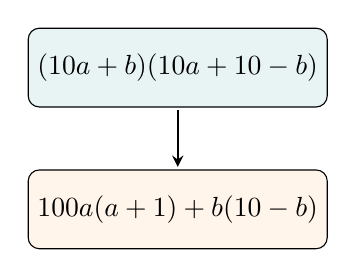
\begin{tikzpicture}[>=stealth,scale=.9]
\node[draw,fill=teal!9,rounded corners,minimum height=1cm] at (4,0){$(10a+b)(10a+10-b)$};
\draw[->,thick] (4,-.6)--(4,-1.4);
\node[draw,fill=orange!8,rounded corners,minimum height=1cm] at (4,-2){$100a(a+1)+b(10-b)$};
\end{tikzpicture}

\end{center}
\medskip
令 $u=10a+5$。写成 $u^2=(u-5)(u+5)+5^2$，得到 $10a(10a+10)+25=100a(a+1)+25$。因此高位 $a(a+1)$，低两位永远 $25$。
\end{explanationbox}
\clearpage
\begin{explanationbox}
\textbf{\textcolor{CExplanation}{首同尾合十与尾数5是同一条规律}}
\par\medskip
\begin{center}
% F088｜pair 原创简明教学示意图
\begin{tikzpicture}[>=stealth,scale=.95]
\node[draw,fill=teal!8,rounded corners] (a) at (0,0) {$23\times27$};
\node[draw,fill=orange!8,rounded corners] (b) at (4,0) {$2\times3\mid3\times7$};
\node[draw,fill=teal!15,rounded corners] (c) at (8,0) {$621$};
\draw[->] (a)--(b);\draw[->] (b)--(c);
\node at (4,-1){\small 十位相同，个位和为 $10$};
\end{tikzpicture}

\end{center}
\medskip
把 $(10a+b)(10a+10-b)$ 看成 $(10a+5-(5-b))(10a+5+(5-b))$。用平方差可得 $100a(a+1)+b(10-b)$。当 $b=5$，两数相同，就回到末位为5的平方。
\end{explanationbox}
\clearpage
\begin{explanationbox}
\textbf{\textcolor{CExplanation}{用数字感受低两位}}
\par\medskip
\begin{center}
% F088｜guard 原创简明教学示意图
\begin{tikzpicture}[>=stealth,scale=.9]
\node[draw,rounded corners,fill=teal!9] at (0,0){$42\times48$};
\node at (3.6,0){$\rightarrow$};
\node[draw,rounded corners,fill=orange!10] at (7,0){$4\times5\mid2\times8$};
\node at (3.6,-1){\small 小尾数乘积不足两位时，要补 $0$};
\end{tikzpicture}

\end{center}
\medskip
个位互补 $b$ 和 $10-b$，它们的积不超过 $25$，一定能放在后两位，不与前面的 $100a(a+1)$ 发生混淆。若 $b=1$，后两位必须写成 $09$ 而不是 $9$。
\end{explanationbox}
